\DiaryEntry{Certain Nonlinear Diophantine Equations}{2023-03-28}{Number Theory}

Coming from \cite{Burton2011}, chapter 12.

\subsection{The Equation $x^2 + y^2 = z^2$}

We first consider the equation

\bee
x^2 + y^2 = z^2
\eee

Because the length $z$ of the hypotenuse of a right triangle is related to the lengths $x$ and $y$ of the sides by the famous Pythagorean equation $x^2 + y^2 = z^2$, the search for all positive integers that satisfy  is equivalent to the problem of finding all right triangles with sides of integral length.

A set of integers $(x,y,z)$ is called a \emph{Pythagorean triple} if $x^2 + y^2 = z^2$ and the triple is said to be primitive if $\gcd(x,y,z) = 1$.

Well-known examples of primitive Pythagorean triples are $(3,4,5), (5, 12, 13)$, and $(12, 35, 37)$.

Suppose that $(x,y,z)$ is any Pythagorean triple and $d = \gcd(x,y,z)$. We therefore can write $x = d x_1, y = d y_1, z = d z_1$ with $\gcd(x_1, y_1, z_1) = 1$ and then we have

\bee
x_1^2 + y_1^2 = \frac{x^2 + y^2}{d^2} = \frac{z^2}{d^2} = z_1^2
\eee

so ($x_1, y_1, z_1)$ is a primitive Pythagorean triple. Thus, it is enough to occupy ourselves with finding all primitive Pythagorean triples; any Pythagorean triple can be obtained from a primitive one upon multiplying by a suitable nonzero integer.

We have two more facts about Pythagorean triples.

\begin{theorem}\label{2023-03-28:th1}
If $(x, y, z)$ is a primitive Pythagorean triple, then one of the integers $x$ or $y$ is even, while the other is odd.
\end{theorem}

Proof: If $x$ and $y$ are both even, then $2|x, 2|y$, and $2 | (x^2+y^2)$ or $2|z^2$ from which follows $2|z$. Therefore, $\gcd(x,y,z) \geq 2$, which contradics the assumption that $(x,y,z)$ is is a primitive Pythagorean triple. If both $x$ and $y$ were odd, then $x^2 \equiv 1 \mod 4$ and $y^2 \equiv 1 \mod 4$ (just try it odd for odd $x$), leading to

\bee
z^2 = x^2 + y^2 \equiv 1 \mod 4
\eee

But this is equally impossible, because the square of any integer must be congruent either to $0$ or to $1$ modulo $4$.\qed

In the following, we will choose $x$ to be even and $y$ to be odd. Then $x^2$ is even, $y^2$ is odd. Therefore $z^2$ is odd, and $z$ is odd as well. We can choose even/oddness differently, but exactely one will be even, while the other two will be odd.

By virtue of above theorem, there exist no primitive Pythagorean triple $(x , y, z)$ all of whose values are prime numbers (as one number is even). There are primitive Pythagorean triples in which $z$ and one of $x$ or $y$ is a prime; for instance, $(3, 4, 5)$, $(11, 60, 61), (19, 180, 181)$. It is unknown whether there exist infinitely many such triples.

We have another theorem about when numbers are square.

\begin{theorem}\label{2023-03-28:th2}
If $ab = c^n$, with $\gcd(a,b) = 1$, then $a$ and $b$ are $n$-th powers; i.e. $a=a_1^n$ and $b = b_1^n$.
\end{theorem}

We assume $a,b > 1$ and write down the prime factorization of $a$ and $b$ as

\bee
a = p_1^{k_1} p_2^{k_2} \cdots p_r^{k_r}, \quad b = q_1^{j_1} q_2^{j_2} \cdots q_s^{j_s}
\eee

Because $\gcd(ab) = 1$, no $p_i$ can occur among the $q_i$ and therefore the prime factorization of $ab$ is

\bee
ab  = p_1^{k_1} p_2^{k_2} \cdot p_r^{k_r} q_1^{j_1} q_2^{j_2} \cdots q_s^{j_s}
\eee

Let's suppose that the prime factorization of $c$ is equal to $c = u_1^{l_1} u_2^{l_2} \cdots u_t^{l_t}$ and then $ab = c^n$ becomes

\bee
p_1^{k_1} p_2^{k_2} \cdot p_r^{k_r} q_1^{j_1} q_2^{j_2} \cdots q_s^{j_s} = u_1^{n l_1} u_2^{n l_2} \cdots u_t^{n l_t}
\eee

From this we see that the primes $u_1, \ldots, u_t$ are the $p_1, \ldots,p_r, q_1, \ldots, q_s$ in some order and the $n l_1, \ldots, n l_t$ are the corresponding exponents $k-1, \ldots, k_r, j_1, \ldots, j_s$ (again in some order). From this we conclude that the $k_i$ and $j_i$ must be divisible by $n$. We therefore can define $a_1$ and $b_1$ as

\bee
a_1 = p_1^{k_1 / n} p_2^{k_2 / n} \cdots p_r^{k_r / n}, \quad b_1 = q_1^{j_1 / n} q_2^{j_2 / n} \cdots q_s^{j_s / n}
\eee

and therefore $a_1^n = a, b_1^n = b$. \qed


With all this in place, we can characterize all primitive Pythagorean triples as follows.

\begin{theorem}\label{2023-03-28:th3}
All the solutions to the Pythagorean equation

\bee
x^2 + y^2 = z^2
\eee

satisfying the conditions

\bee
\gcd(x,y,z) = 1, \quad 2 | x, \quad x,y,z > 0
\eee

are given by the formulas

\bee
x = 2st, \quad y = s^2-t^2, \quad z = s^2 + t^2
\eee

for integers $s > t > 0, \gcd(s,t)=1$, and $s \not\equiv t \mod 2$.
\end{theorem}

Proof: Assume that $(x,y,z)$ is a primitive Pythagorean triple. We have chosen $x$ to be even, and $y,z,$ as odd. Therefore $z-y$ and $z+y$ are even; define $z-y=2u$ and $z+y=2v$. Let's rewrite $x^2+y^2=z^2$ as

\bee
x^2 = z^2 - y^2 = (z-y)(z+y)
\eee

and therefore

\bee
\left( \frac{x}{2} \right)^2 = \left( \frac{z-y}{2} \right) \left( \frac{z+y}{2} \right)^2 = uv
\eee

We notice that $u$ and $v$ are relatively prime; if $\gcd(u,v) = d > 1$, then $d | (u-v)$ and $d | (u+v)$, or $d|y$ and $d|z$, which violates the fact that $\gcd(y,z)=1$. Using the previous theorem, we can express $u, v$ as

\bee
u=t^2, \quad v = s^2
\eee

where $s$ and $t$ are positive integers. Substituting everything back yields

\begin{align*}
z &= u + v = s^2 + t^2 \\
y &= v - u = s^2 - t^2 \\
x^2 &= 4uv = 4s^2t^2 \rightarrow x = 2st
\end{align*}

A common factor of $s$ and $t$ would also divide both $y$ and $z$; the condition $\gcd(y,z) = 1$ forces $\gcd(s,t) = 1$. Finally, we observe that if $s$ and $t$ were both even or both odd, then this would make both $y$ and $z$ even which is not possible. Hence, one of the pair $s,t$ is even, the oher is odd - this can also be written as $s \not\equiv t \mod 2$.

In the other direction, we take $x = 2st, y = s^2-t^2, z = s^2 + t^2$ and check that

\bee
x^2 + y^2 = (2st)^2 + (s^2-t^2)^2 = (s^2 + t^2)^2 = z^2
\eee

To see that this triple is primitive, we assume that $\gcd(x,y,z) = d > 1$ and take $p$ to be any prime divisor of $d$. We must have $p \neq 2$ because $p$ divides the odd integer $z$ (one of $s$ and $t$ is odd, the other even, and therefore $z = s^2 + t^2$ must be odd). From $p | y$ and $p|z$, we obtain $p | (z+y)$ and $p | (z-y)$. From the definitions $y = s^2-t^2, z = s^2 + t^2$ follow $z+y=2s^2$ and $z-y=2t^2$ and therefore $p|2s^2$ and $p|2t^2$. But then $p|s$ and $p|t$ and this is incompatible with $\gcd(s,t)=1$. To resolve this contradiction, we must have $d=1$ and $(x,y,z)$ contitutes a primitive Pythagorean triple. \qed

The following screenshot shows a table with some Pythagorean triples. For each value of $s$, we have taken those values of $t$ that are relatively prime to $s$, less than $s$, and even whenever $s$ is odd.

\begin{figure}[H]
    \centering
    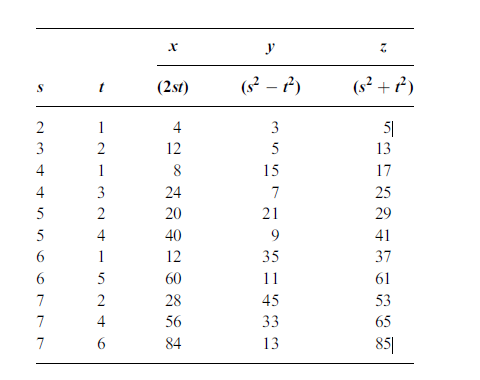
\includegraphics[scale=0.75]{images/2023-03-28-triples.png}
\end{figure}

Looking at this, we suspect that if $(x , y, z)$ is a primitive Pythagorean triple, then exactly one of the integers $x$ or $y$ is divisible by $3$. According to the previous theorem, we have $x=st, y=s^2-t^2, z=s^2+t^2$ with $\gcd(s,t)=1$, If either $3|s$ or $3|t$, then $3|x$ and we are done. Now consider the case that $3 \nmid s$ and $3 \nmid t$. That is, we can write $s = 3k+1$ or $s=3k+2$. In the first case, $s^2 =  9k^2 + 6k + 1 \equiv 1 \mod 3$; in the latter case, $s^2 = 9k^2 + 12k + 4 \equiv 1 \mod 3$. Therefore, $y = s^2 - t^2 \equiv 0 \mod 3$. So, $y$ is divisible by $3$. \qed

\paragraph{Problem 12.1} a) Find Pythagorean triples (not necessarily primitive) of the form $(16,y,z)$.

We start by $x= 2st$ from Theorem \ref{2023-03-28:th3} from which we obtain $st = 8$. The easiest way is to enumerate all $(s,t)$; however, we have to keep in mind that $s > t > 0$ and $\gcd(s,t) = 1$. There are not many left, in fact only the pair $(s=8, t=1)$. From this follows $y = s^2 - t^2 = 63$ and $z = s^2 + t^2 = 65$ and our first primitive triple is $(16, 63, 65)$. Since there are no other $(s,t)$ combinations possible, we have to find non-primitive Pythagorean triples and multiply them with some factor to obtain a triple of the desired form $(16, y, z)$.

Let's start with triples of the form $(2, y, z)$: We have $2st = 2 \rightarrow st = 1$ but conditions $s > t > 0$ and $\gcd(s,t) = 1$ forbid any solution. Let's consider $(4, y, z)$ instead: $2st = 4 \rightarrow st = 2$ and this is only fulfilled by $s = 2, t=1$. From this follows the triple $(4,3,5)$. Now we multiply with $4$ and obtain the non-trivial triple $(16, 12, 20)$. Another triple can be found based on the primitive triple $(8, y, z)$. Here, $st=4 \rightarrow s = 4, t=1$, and we obtain $(8, 15, 17)$ which becomes $(16, 30, 34)$ by multiplication with $2$. \qed

The b) part is finding primitive Pythagorean triples of the form $(40,y,z)$ and $(60,y,z)$. Nothing fancy to be seen here; basically, we have $2st = 40$, then we list all valid $(s,t)$ combinations and calculate $y$ and $z$ of these (like done above) - that's it.

\paragraph{Problem 6} Show that $(3,4,5)$ is the only primitive Pythagorean triple involving consecutive positive integers. We can write this down as

\bee
x^2 + (x+1)^2 = (x+2)^2 \rightarrow x^2 - 2x - 3 = 0
\eee

and we can solve this quadratic equation as

\bee
x_{1,2} = 1 \pm \sqrt{1+3} = 1 \pm 2 = \begin{cases} &3 \\ &-1 \end{cases}
\eee

Only the positive solution makes sense and this is exactely $(3,4,5)$. Multiplying this triple by some number $k$ yields a non-primitive Pythagorean triple and this won't have consecutive integers; e.g. $(6, 8, 10)$, so $(3,4,5)$ is the only one.

\paragraph{Problem 9} a) Prove that if $(x , y, z)$ is a primitive Pythagorean triple in which $x$ and $z$ are consecutive positive integers, then

\bee
x = 2t(t+1), \quad y = 2t+1 \quad z = 2t(t+1)+1
\eee

for some $t > 0$. We start by noting that $z - x = 1 = s^2+t^2 - 2st = (s-t)^2$ from which follows $s - t = 1$ or $s = t+1$. Inserting this into $x = 2st$ yields $x = 2t(t+1)$ and $y = s^2-t^2 = (t+1)^2 - t^2 = 2t+1$. Finally, $z = x+1 = st(t+1)+1$. \qed

For $t=1$, this yields $(3,4,5)$, for $t=$ we obtain $(12, 5, 13)$.

b) Prove that if $(x , y, z)$ is a primitive Pythagorean triple in which the difference $z-y = 2$, then

\bee
x = 2t, \quad y = t^2-1, \quad z = t^2+1
\eee

for some $t > 1$. From $z - y = 2 = s^2+t^2 - (s^2 - t^2) = 2t^2$ we have $t = 1$. So $x = 2st = 2s, y = s^2-t^2 = s^2-1, z = s^2 + t^2 = s^2 + 1$. \qed

For $s=2$ this yields our well-known $(3,4,5)$, for $s=3$ we obtain $(6,8,10)$, but this is \emph{not} a Pythagorean triple. Be careful - the statement works in the direction "Pythagorean triple" $\rightarrow$ "express $x,y,z$ as ... and \emph{not the other way round}. For $s=4$ the formulas give a Pythagorean triple, $(8, 15, 17)$.


%%% Local Variables:
%%% mode: latex
%%% TeX-master: "journal"
%%% End:
